\documentclass[../main.tex]{subfiles}
\begin{document} \label{chapter_hmms}

Having extracted formant trajectories, our goal is now to build a more abstract structure that summarises their shape and content. This reflects the need to measure the similarity of the trajectories symbolically, rather than as sequences of varying length. Once any such structure has been trained, a similarity measure can be used to create a distance matrix, which serves as input to the relational structure building algorithms described in section \ref{algorithms_review}.
\par We first discuss statistical models to represent formant trajectories. In section \ref{section_kde}, we describe a method to generate a discrete probability distributions as a linear combination of basis functions. After, in section \ref{subsection_gmm}, we generalise this discussion to model formant trajectories as a mixture of Gaussians. This allows us to introduce latent variables, i.e. to explicitly let the content formant trajectories be described
as a mixture of hidden parametrised distributions.
\par In section \ref{section_hmm}, we further extend the discussion to models that allow learning of time-ordered sequences: Hidden Markov Models. In particular, we do not only discuss the concept of HMMs, but we also touch on Bayesian Inference, a powerful concept that allows us to do fully probabilistic learning. Next, we discuss Approximate
Inference, which is a method to perform Bayesian Inference over models with latent variables, where full Bayesian Inference often becomes intractable.
\par We then present similarity metrics between the statistical models presented in this chapter, in section \ref{section_similarity}. These enable us to perform agglomerative hierarchical clustering, which we touched on first in chapter \ref{chapter_soa}. We give a deeper discussion on this technique in section \ref{section_hierarchical}.


\section{Kernel density estimation} \label{section_kde}
In this section, we describe Kernel Density Estimation. We focus the discussion on the unidimensional case (for reasons that will become clearer in chapter \ref{chapter_account}), and refer the reader to the cited works for the multivariate case. 
\par Given a continuous distribution $F(x)$ with density $\frac{d}{dx}F(x) = f(x)$, the goal is to estimate $f(x)$ from a finite sample $X = \{x_1, x_2, ..., x_N\}$ \cite{Hansen2009}. 
\par The most basic approach to build probability distributions is to use histograms. Histograms are built by dividing an interval into $M$ bins of not-necessarily-equal width, counting how many points fall within each bin, and normalising these quantities so that the resultant becomes a probability distribution. We first generate a vector $B = (b_0, b_1, b_2, ..., b_M)$, where $b_{i+1} - b_i = w_i, 0 < i \leq M$ is the width of bin $i$ and the $b_i$ are called endpoints. Then, the vector 
\begin{align*}
\V{H} &= (H_i)\\
H_i &= \frac{1}{N}\sum_{j=1}^{N}\frac{\mathbb{I}( b_{i} < x_j \leq b_{i+1})}{w_i}, \forall i \leq M
\end{align*}
is the histogram corresponding to the dataset $X$ for the given endpoints.
\par There are two issues with this approach: on one hand, the histogram function is not smooth, i.e. we are prone to see discontinuities at the edges of each bin; on the other hand, each histogram depends heavily on its endpoints, both in terms of the width of each bin, and in terms of \emph{where} they are located \cite{Duong2004}. This results in having radically different histograms for each selection of endpoints, as can be seen in figure \ref{fig_histograms}.
\begin{figure}[t]
\centering
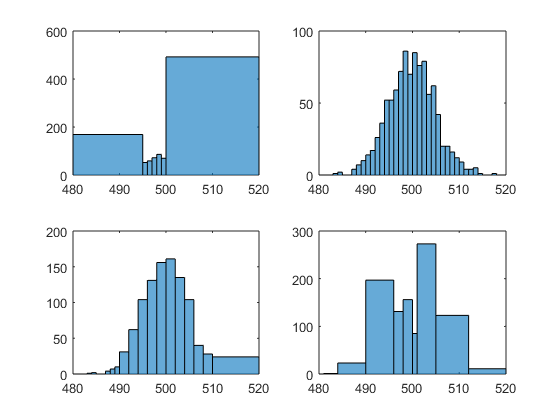
\includegraphics[width=\textwidth]{histograms}
\caption{Four histograms over the same data, with different bin edges in each subplot. Note how the selection of bin edges radically affects the resulting histogram.}
\label{fig_histograms}
\end{figure}
\par We now consider a method that overcomes these issues. To do so, we first remark the following: consider the set of uniform distributions given by $\{\mathcal{U}_i = \mathcal{U}(b_{i}, b_{i+1})\}$. This distribution covers a range of length $w_i = b_{i+1}-b_i$ and is centered in $c_i = \frac{b_{i+1}+b_i}{2}$.  Let $h_i = \frac{w_i}{2}$ and notice that anytime $\abs{x_j - c_i} \leq h_i$, or equivalently,
\begin{align*}
\left|\frac{x_j - c_i}{h_i}\right| \leq 1
\end{align*}
\par then an instance of the uniform distribution $\mathcal{U}_i(x) = \frac{\mathbb{I}(b_i < x \leq b_{i+1})}{2h_i}$ is ``stacked" over $c_i$. To summarise, we can conclude that the histogram probability distribution can be modelled equivalently as:
\begin{align*}
p_H(x) = \frac{1}{N}\sum_{i=1}^M\frac{1}{2h_i}\mathbb{I}\left(\left|\frac{x - c_i}{h_i}\right| \leq 1\right)
\end{align*}
\par In other words, we have an asset of $N$ uniform distributions centered at each $c_i$; by additivity of integration, the total area under these distributions is equal to $N$, and thus we just have to normalise by dividing over $N$ to make this linear combination a new probability distribution. Now, assume that we let each uniform distribution $\mathcal{U}_i$ have the same width, and that we center each uniform distribution at each $x_j \in X$, i.e. now we have $N$ overlapping bins. Then, the expression above becomes:
\begin{align*}
p_{H}(x) &= \frac{1}{N}\sum_{j=1}^N\frac{1}{2h}\mathbb{I}\left(\left|\frac{x - x_j}{h}\right| \leq 1\right)\\
&= \frac{1}{Nh}\sum_{j=1}^NK_u(\left|\frac{x - x_j}{h}\right|),\\
K_u(x) &= \left\{
     \begin{array}{lr}
      \frac{1}{2} & \abs{x} \leq 1 \\
      0 & \text{otherwise} 
     \end{array}
   \right.
\end{align*}
\par This function no longer represente¿s a histogram, but rather a staircase pyramid, as shown in figure \ref{fig_hist2}. Moreover, we also notice that we have transformed our original expression so as to make it depend on a very well known function, the uniform kernel $K_u$ \cite{Hansen2009}. 
\begin{figure}[t]
\centering
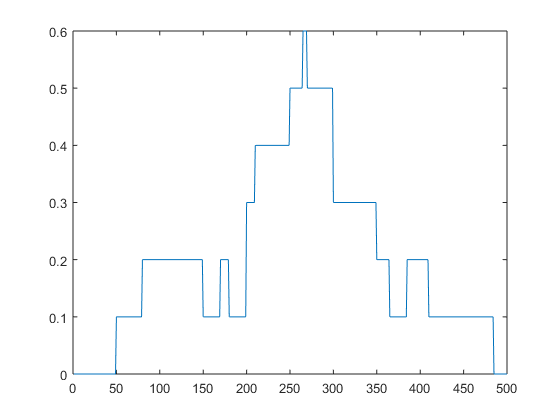
\includegraphics[width=80mm]{histogram2}
\caption{The probability distribution generated by placing uniform distributions of the same width along the $x$ axis, centered around each data point $x_j$.}
\label{fig_hist2}
\end{figure}
\par Although this function is not smooth, we can now use the fact that it depends on the kernel $K_u(x)$, and think of the latter as a basis function used to shape the resulting density. We recall that a kernel is any function that integrates to one, i.e. $\int_{-\infty}^\infty K(x)dx = 1$. A non-negative kernel $K$ is one such that $K(x) \geq 0 \forall x$, in which case $K$ is a probability distribution \cite{Hansen2009}.
\par This concept is referred to as Kernel Density Estimation: it can approximate the probability density function of a set of points as a weighted linear combination of basis functions (non-negative kernels). 
\begin{align*}
p_K(x) = \frac{1}{Nh}\sum_{i=1}^NK\left(\left|\frac{x - x_i}{h}\right|\right),\\
\end{align*}
\par Furthermore, instead of using the uniform kernel, we can use a smooth kernel and hence (given that the sum $f+g$ of two continuous functions $f, g: \mathbb{R} \rightarrow \mathbb{R}$ is continuous) obtain a smooth probability function. 
\par Using a smooth kernel provides a smooth probability function as a result. However, this still does not solve the issue with the width parameter $h$ (reffered to as the kernel \emph{bandwidth}). The bandwidth $h$ controls the degree of smoothness of the curve, and thus tuning it is crucial in order to get accurate results. The resulting probability function could be oversmoothed, undersmoothed or optimally smoothed, as is depicted in figure \ref{fig_kdebandwidths}, depending on the value of $h$ \cite{Duong2004}.
\begin{figure}[t]
\centering
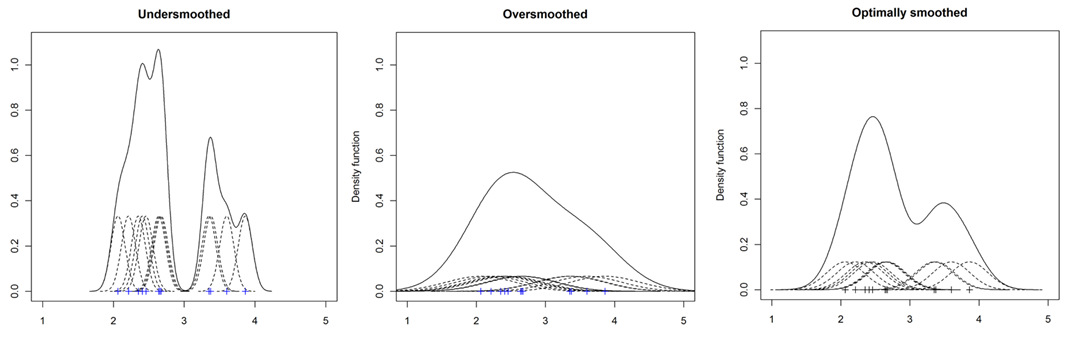
\includegraphics[width=\textwidth]{kdebandwidth}
\caption{Three probability density functions fitted using KDE with Gaussian kernels and different bandwidths. Images retrieved from \cite{Duong2004}.}
\label{fig_kdebandwidths}
\end{figure}
\par One of the most common smooth kernels in the literature is the Gaussian kernel \cite{hastie2008}, given by:
\begin{align*}
K_G\left(\frac{x}{h}\right) = \frac{1}{\sqrt{2\pi}}\exp{\{-\frac{x^2}{2h^2}\}}
\end{align*}
\par Its popularity is due not only to its close relationship to the Normal distribution (KDE places small Gaussians centered in each datapoint in this case), but also because there is a rule of thumb on how to set the bandwidth $h$. The details of the derivation for this rule are out of the scope of this work, but can be consulted in \cite{Hansen2009}. In particular, for univariate Gaussians, the optimal bandwidth in the least-squares error sense is given by $h = \hat{\sigma}n^{-1/5}$, where $\hat{\sigma}$ is the standard deviation of the sample $X$.
\par Note that, despite its simplicity, KDE is a poorly scalable strategy: on one hand, the bandwidth $h$ becomes harder to choose as the dimensionality of data increases \cite{Hansen2009}; on the other hand, the number of points to be stored increases exponentially with each added dimension.

\section{Gaussian Mixture Models}\label{subsection_gmm}
The scalability challenge imposed by KDE motivates the look for a more compact representation of data. Moreover, formant trajectories for different birdsong syllables from the same species have been shown to exist in different frequency ranges. This suggests the existence of subpopulations in our data $\mathcal{X}$. Moreover, it also suggests that the data can be explained by a model with fewer basis functions than KDE. In particular, assume that there exist $K$ subpopulations $\mathcal{X}_i$ in our data. Then, if every subpopulation is assumed to be drawn from the same distribution, the probability of the whole data $\mathcal{X}$ can be seen as a \emph{mixture} of $K$ components $p_i$ \cite{Murphy2012}:
\begin{equation} \label{eq:mixmod}
p(\V{x} \given \theta ) = \sum_{i=1}^K\pi_i p_i(\V{x} \given \theta_i)
\end{equation}
Where $p_i$ represents the $i$-th component with parameters $\theta_i$ and $\pi_i$ is the weight of component $p_i$. The weights satisfy $0 \leq \pi_i \leq 1 \forall i, \sum_i \pi_i = 1$. By letting all $p_i$ be Normal distributions, we obtain a Gaussian Mixture Model (GMM) \cite{Bishop2006}:
\begin{equation*} \label{eq:gmm}
p_i(\V{x} \given \theta) = \mathcal{N}(\V{\mu}_i, \Sigma_i) \forall i
\end{equation*}
An example of a GMM fitted to a dataset comprising three subpopulations is shown in figure \ref{fig_gmm}. By fitting a 3-mixture GMM, we can see that each component corresponds with each subpopulation in the dataset.
\par Additionally, this new model also overcomes some of the scalability issues of KDE. By introducing parameters, we are bounding the amount of storage needed for the model. For a GMM, the resources needed grow linearly on $K$ to store mean vectors $\mu$ and quadratically on $K$ to store covariance matrices $\Sigma$. However, this improvement comes at the expense of a harder training procedure. Additionally, although we have removed the selection of the bandwidth $h$ from KDE, we now have to choose the number of components $K$ in the mixture.
\par Furthermore, note that the usage of mixture models induces the existence of hidden variables: before training the mixture model, we assume that $K$ unknown components $s_i$ generated the data. This allows us to rewrite the $i$-th mixture as $p_i(x) = p(x \given s_i)$, i.e. given a mixture, that probability of drawing $x$ from it is exactly the probability given by mixture $p_i$. 
\par However, there is still one issue with GMMs. Although they are more scalable than KDE, neither KDE nor GMMs allow for the existence of time ordering of data. In other words, both models treat the formant trajectories as sets, hence losing the structural sequence they originally were. In this project, this would imply that two bird species whose formant trajectories are always in the same range would not be distinguishable, even if the syllables they produce were different in shape. This motivates the need for an even more abstract structure that takes into consideration the sequential structure of formant trajectories.

\begin{figure}[t]
\centering
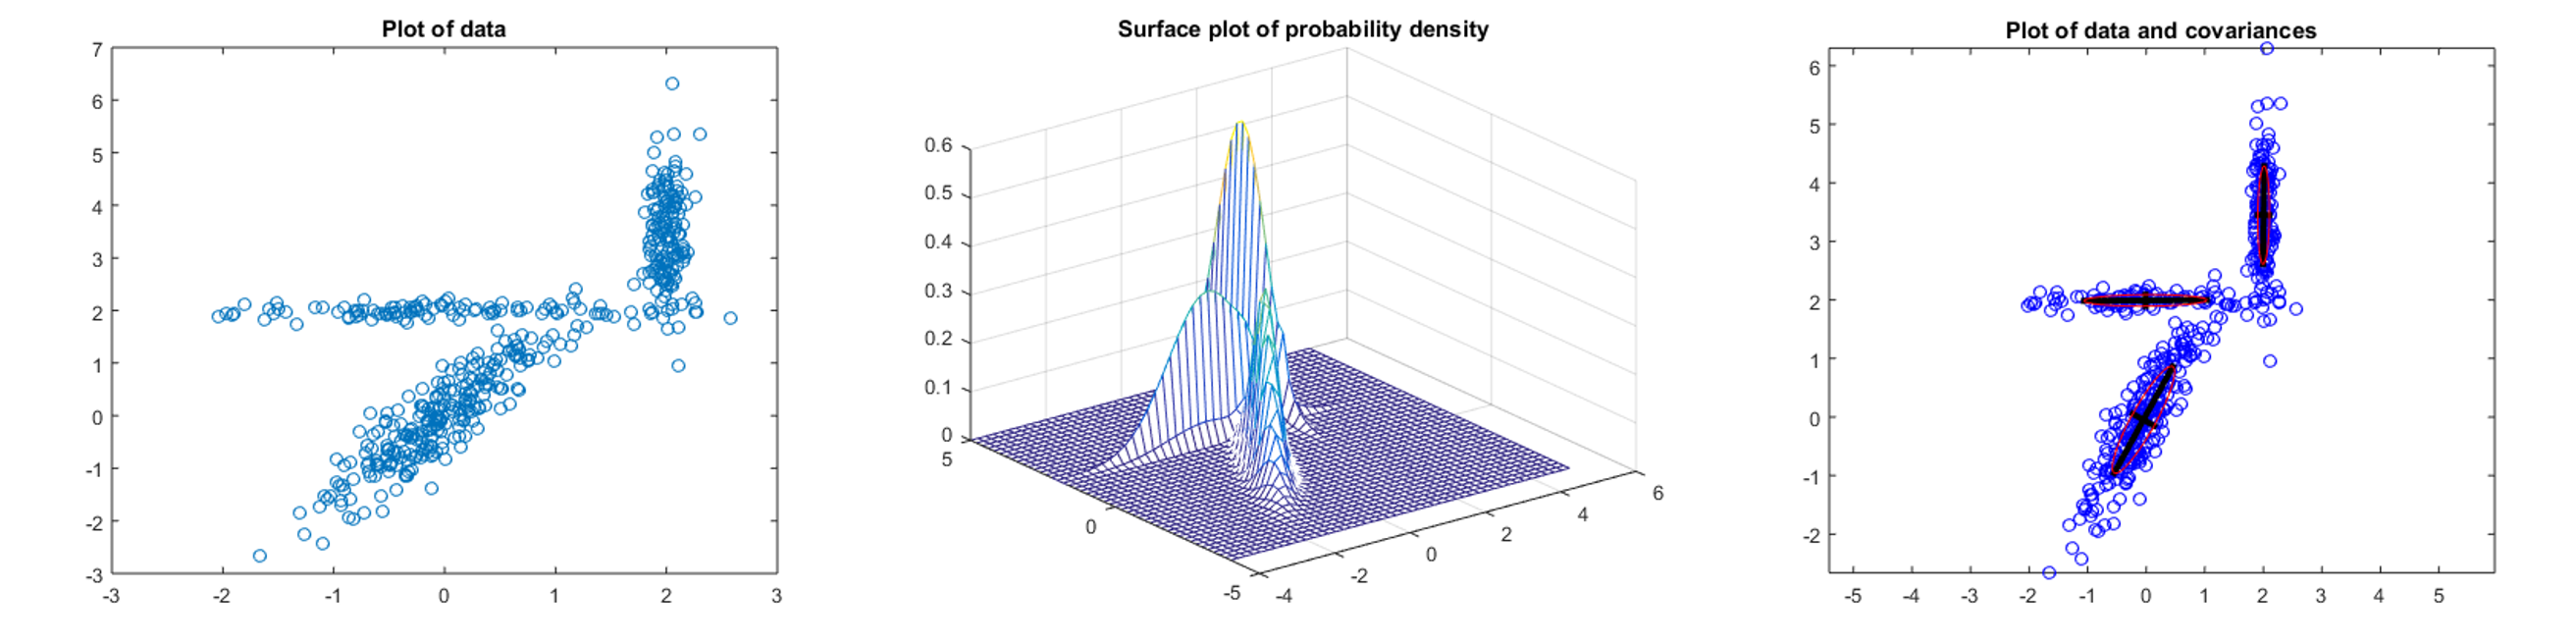
\includegraphics[width=\textwidth]{gmm}
\caption{Left: data drawn from three normal distributions. Middle: GMM surface with three components fitting the data. Right: level curve of each GMM component over the subpopulation it represents. These images were generated using the NETLAB toolbox.}
\label{fig_gmm}
\end{figure}

\section{Hidden Markov Models} \label{section_hmm}
In this section, we address the issues discussed in section \ref{subsection_gmm}. Although Gaussian Mixture Models overcome the scalability issues of KDE, both techniques still suffer from losing the sequential structure of formant trajectories. Hidden Markov Models overcome these challenges by combining an \emph{emission model} with a \emph{transition model}, i.e. given a sequence $\V{x}$, the emission model explains the observations in the sequence, whereas the transition model explains the sequential structure of data. 
\par In subsection \ref{subsection_defhmms}, we aim to define Hidden Markov Models. To this end, we introduce the concept of Markov chains and then generalise them to offer a full definition of Hidden Markov Models.
\par HMMs, like GMMs, are hidden (latent) variable models. This means that we have to choose a number of components that help explaining the data. Moreover, we have yet to describe a training procedure to obtain a model that explains data. These two challenges are touched on in subsection \ref{subsection_model}, where we introduce Approximate Bayesian inference. This is a learning approach that avoids the computational complexity of sample-based Bayesian inference in complex models while also deciding the optimal number of components $K$ in an HMM.

\subsection{Definition} \label{subsection_defhmms}
In this subsection, we introduce the theory behind Hidden Markov Models. We first present the more general concept of Markov chain, which will allow us to introduce HMMs more naturally. 
\par Assume that a system is in a state $s_t$ from a set $Q = \{ q_1, q_2, ..., q_K \}$ at time $t$, and that we observe the system periodically so as to obtain a sequence $\V{s} = \left( s_1, s_2, ..., s_T \right)$, where $s_t \in Q$. Note that we are able to confirm that the state of the system $s_t$ is at any time $t$. Furthermore, assume that the state the system reaches at $t+1$, $s_{t+1}$, only depends on where it was one time step before, $s_t$. That is, $s_{t+1}$ is conditional only on $s_{t}$, and does not go further back in time to make a decision. Then, we say that the system satisfies the \emph{Markov property} \cite{Murphy2012}.
\par A Markov chain models the transition probabilities $p(s_{t+1} \given s_t)$ of a system satisfying the Markov Property. By the product rule, we can model the probability that a given sequence was generated by the system as:
\begin{equation}\label{eq:chain}
p(\V{s}) = p(s_1)\prod_{t=1}^{T-1}p(s_{t+1} \given s_t)
\end{equation}
\par Nevertheless, it is not always true that we are able to observe the state of the system of study: some systems might have a  hidden Markov process for which we can only obtain a sequence of observations $\V{x} = \left( \V{x}_1, \V{x}_2, ..., \V{x}_T \right)$, but not its associated state sequence $\V{s}$. Because we cannot directly observe what state the system is in, we can only say that a particular observation $\V{x}_t$ is generated by state $\V{s}_t$ with probability $p(\V{x}_t \given \V{s}_t)$ \cite{Murphy2012}. 
\par In this scenario, we aim to infer the probability that the model generated such observations $\V{x}$ and that the underlying Markov Process generated the sequence of states $\V{s}$. This is given by the joint probability $p(\V{x}, \V{s})$, which can be expanded in terms of equation \ref{eq:chain}.
\begin{equation}\label{eq:hmm}
p(\V{x}, \V{s}) = p(\V{s})p(\V{x} \given \V{s}) = p(s_1)\prod_{t=1}^{T-1}p(s_{t+1}\given s_t)\prod_{t=1}^Tp(\V{x}_t \given s_t)
\end{equation} 
\par A Hidden Markov Model is a statistical tool that models the scenario presented above, in which we observe a sequence $\V{x}$ associated to a sequence of latent states $\V{s}$ and then want to infer, for example \cite{Jurafsky2009, Bishop2006}: given a sequence of observations $\V{x}$ and an HMM, what is the sequence of states $\V{s}$ that most likely generated $\V{x}$? Or: given a sequence of observations $\V{x}$ and a sequence of states $\V{s}$, what is the probability $p(\V{x} \given \V{s})$ that $\V{s}$ generated $\V{x}$?  
\par From equation \ref{eq:hmm} we note three key elements \cite{Ghahramani2001}: the factor $p(s_1)$ is the probability of starting the process in state $q_k \in Q$, and therefore is a associated to a distribution $\pi(q_k)$ over the states $Q$. This is called the \emph{initial state distribution}. Next, the transition probabilities $p(s_{t+1} \given s_t)$ are associated to a Markov chain describing the probabilities $p(q_j \given q_i)$, i.e. going from state $q_j$ to state $q_i$. This is called the \emph{transition model}, and is described by a matrix $A$ with entries $a_{i,j} = p(q_j \given q_i)$. Finally, the observations are linked to a distribution $p(\V{x}_t \given s_t)$ called the \emph{observation} or \emph{emission model}, with parameters $\phi$. 
\par An HMM is fully characterised (up to a permutation of states) by these three parameters $\theta = (\phi, B, \pi)$. Furthermore, the observations analysed by an HMM can be continuous or discrete \cite{Jurafsky2009}. Note that formants $\V{f}_i$ belong to a continuous space, hence we will focus on describing continuous HMMs henceforth.
\par Let the emission model of an HMM be a GMM. Notice that the transition model explains the data's sequential structure without losing any of the GMM's advantages described in section \ref{subsection_gmm}. Thus we have overcome the main challenge described for GMMs. However, we still have two matters to address: on one hand, we have yet to describe a learning procedure for continuous HMMs; on the other hand, we also have to touch on model selection, i.e. finding a method to choose how many states should an HMM have. Both of these issues are discussed in subsection \ref{subsection_model}.
\par Finally, note that for every HMM with $K$ states, there exist $K!$ equivalent HMMs that can be generated by permuting the identities of the HMM's states. This problem is called \emph{identifiability} \cite{Bishop2006}, and will play an important role when we define a metric between HMMs. 

\subsection{Training and model selection} \label{subsection_model}
Given the description of HMMs from subsection \ref{subsection_defhmms}, two questions arise naturally: first, given a sequence $\V{x}$, how do we \emph{train} an HMM, i.e. how do we describe the parameters $\theta = (A, \phi, \pi)$? And second: how do we choose the number of states $K$ the HMM should have?
\par We first address HMM training. We aim to make inferences about the parameters $\theta$ given data $\mathcal{X}$. This is captured by the \emph{posterior probability}, given by $p(\theta \given \mathcal{X})$. The posterior summarises everything we know about the parameters of the model, i.e. it measures the uncertainty of the parameters given data $\emph{X}$, and it can be expanded by Bayes' Theorem as:
\begin{equation}\label{eq:bayes_posterior}
p(\theta \given \mathcal{X}) = \frac{p(\mathcal{X} \given \theta)p(\theta)}{p(\mathcal{X})}
\end{equation}
\par The factor $p(\mathcal{X} \given \theta)$ is called the \emph{likelihood}, and corresponds to the probability of seeing the data generated by a model with parameters $\theta$. The \emph{prior distribution} is given by $p(\theta)$, and it describes our beliefs about the posterior before seeing the data. Finally, the factor $p(\mathcal{X})$ is called the \emph{marginal likelihood}, and it can be seen as a normalising constant. 
\par A \emph{frequentist} approach to learning (i.e. one that assumes that probability can be seen as how frequently an event would happen if we could sample an infinite number of times) is Maximum Likelihood Estimation (MLE). MLE consists in finding a point estimate $\hat{\theta}$ that maximises the likelihood $p(\mathcal{X} \given \theta)$, i.e.
\begin{equation}
\hat{\theta} = \argmax{p(\mathcal{X} \given \theta)}
\end{equation}
\par However, MLE has several disadvantages \cite{Murphy2012}. Firstly, there is no measure of uncertainty regarding the point estimate $\hat{\theta}$, and thus we are not able to know how trustworthy the estimate is. Secondly, the mode of a distribution is often untypical of the distribution \cite{Murphy2012} because it does not take into account the volume distribution of the probability distribution. Finally, MLE estimates are prone to overfit data. To illustrate this scenario, consider a fair coin that is tossed two times, and it lands heads on both occasions. An MLE estimate for this Bernoulli distribution would set $\hat{\theta} = 1$, i.e. it would immediately conclude that the coin is loaded \cite{Murphy2012}.
\par These disadvantages can be treated by performing full probabilistic (Bayesian) learning. In the Bayesian approach, we measure uncertainty by letting the parameters $\theta$ be probability distributions about which we have beliefs. These are represented by prior distributions. Although the inclusion of beliefs as prior distributions has been the cause of much controversy in the Machine Learning community, it is always possible to use \emph{uninformative priors} to reduce the impact of the prior in the resultant distribution \cite{Bishop2006}. 
\par The following discussion is based on \cite{Ghahramani2001,Beal2003}. Consider using Bayesian inference to learn a model with latent variables. Then, the marginal likelihood is given by marginalising over $\theta$ and the latent variables $\V{s}$:
\begin{align*}
p(\V{x} \given m) &= \int\int p(\V{x}, \V{s}, \theta \given m) d\V{x} d\theta
\end{align*}
\par This integral is often intractable, which implies that a fully Bayesian treatment cannot be done. In this case, we try to make an approximation by means of the Variational Bayes (VB) framework. Consider the log-marginal likelihood $\log{p(\V{x} \given m)}$ for the same model:
\begin{align*}\label{eq:marginal}
\log{p(\V{x} \given m)} &= \log{\int\int p(\V{x}, \V{s}, \theta \given m) d\V{x} d\theta}\\
&= \log{\int\int \frac{q(\V{s}, \theta)}{q(\V{s}, \theta)}p(\V{x}, \V{s}, \theta \given m) d\V{x} d\theta}
\end{align*}
by Jensen's inequality:
\begin{equation*}\label{eq:jensen}
\log{p(\V{x} \given m)} \geq  \int\int q(\V{s}, \theta)\log{\frac{p(\V{x}, \V{s}, \theta \given m)}{q(\V{s}, \theta)}} d\V{x} d\theta
\end{equation*}
Maximising this lower bound with respect to the free distribution $q(\V{s}, \theta)$ yields $q(\V{s}, \theta) = p(\V{s}, \theta \given \V{x}, m)$, i.e. the posterior distribution. Now assume that we can factorise $q(\V{s}, \theta) \approx q_{\V{s}}(\V{s})q_{\theta}(\theta)$ (mean field assumption \cite{Rezek2005}). Then:
\begin{align*}
\log{p(\V{x} \given m)} &\geq  \int\int q_{\V{s}}(\V{s})q_{\theta}(\theta)\log{\frac{p(\V{x}, \V{s}, \theta \given m)}{q_{\V{s}}(\V{s})q_{\theta}(\theta)}} d\V{x} d\theta \\
 &= \mathcal{F}_m(q_{\V{s}}(\V{s}), q_{\theta}(\theta), \V{x})
\end{align*}
Remark that $F_m$ is a functional (i.e. a mapping from a function to a scalar). Using the calculus of variations, we can optimise $F_m$ with respect to $q_{\V{s}}(\V{s})q_{\theta}(\theta)$ simultaneously and arrive at alternating update equations:
\begin{align*}
q_{\V{s}}^{(t+1)}(\V{s}) &\propto \exp{ \bigg[ \int \log{p(\V{x}, \V{s} \given \theta, m)} q_\theta^t(\theta) d\theta \bigg] } \\
q_{\theta}^{(t+1)}(\theta) &\propto p(\theta \given m) \exp{\bigg[ \int \log{p(\V{x}, \V{s} \given \theta, m)} q_{\V{s}}^{t+1}(\V{s}))d\V{s} \bigg]}
\end{align*}
Furthermore, it can be proved that the following holds:
\begin{align*}
\log{p(\V{x} \given m)} - \mathcal{F}_m(q_{\V{s}}(\V{s}), q_{\theta}(\theta), \V{x}) &= \int\int q_{\V{s}}(\V{s})q_{\theta}(\theta)\log{\frac{q_{\V{s}}(\V{s})q_{\theta}(\theta)}{p(\V{x}, \V{s}, \theta \given m)}} d\V{x} d\theta\\ &= \text{KL}\infdiv{q}{p}
\end{align*}
\par In other words, finding the distributions $q_\V{s}, q_\theta$ that best approximate the true posterior by maximising $\mathcal{F}_m$ is equivalent to minimising the KL-divergence between the approximation $q(\V{s}, \theta)$ and the true posterior $p(\V{s}, \theta \given \V{x}, m)$ \cite{Ghahramani2003}. This iterative procedure resembles the EM algorithm (the MLE approach to train models with latent variables), in the sense that we make alternating updates to estimate our beliefs about the parameters.
\par Additionally, notice that the update equation for $q_{\theta}^{(t+1)}(\theta)$ makes use of the prior distribution described in equation \ref{eq:bayes_posterior}. The prior distribution is a key component in VB because it enables us to include our beliefs about the model's parameters prior to seeing the data \cite{Genovese2004}. Moreover, recall that $\text{posterior} \propto \text{likelihood} \times \text{prior}$. It turns out that, for specific combinations of likelihood and prior densities, the posterior and the prior are conjugate, i.e. they belong to the same family of models \cite{Rezek2005}. For example, a Dirichlet prior is conjugate for a multinomial likelihood, and thus the posterior of the model is a Dirichlet distribution. 
\par A full treatment of how the VB framework can be used for continuous HMM training is given in \cite{Rezek2005}, and further details for discrete HMMs can also be found in \cite{Beal2001,MacKay1997}. In \cite{Rezek2005}, the authors approximate the posterior distributions for the transition and HMM initial state probabilities as Dirichlet distributions, and give an account of the models for different kinds of observations. In particular, for Gaussian observation models, they approximate the mean as a Normal Distribution and the precision matrices as Wishart densities. Further details on the parameters and update equations for them can be found in their work. The reader is referred to appendix \ref{subsection_dirwish} for further details on the Dirichlet and Wishart distributions.
\par Having discussed VB HMM training, there is only one issue to address: model selection, i.e. determining how many states an HMM should have. Although techniques such as cross-validation have been investigated \cite{Siddiqi2007,Rezek2005} to choose the number of states $K$, VB approaches have been shown a natural shrinkage of the number of states, i.e. the state space dimension $K$ need not be estimated by iterative training and testing of models. Instead, the system accounts a natural shrinkage: states not visited by the model collapse and only those that correspond to the true number of clusters are used \cite{Rezek2005}. 

\subsection{Conclusion}
In this section, we presented Hidden Markov Models, which are capable of modelling sequentially structured data. Moreover, we addressed the issues of training and model selection by describing the Variational Bayes framework, which treats parameters as probability distributions (rather than point estimates) and hence enables us to quantify their uncertainty. The next step is to find a way to define similarity between the statistical models described in this section and in sections \ref{section_kde} and \ref{subsection_gmm}. This will allow us to create a relational structure by means of agglomerative hierarchical clustering.

\section{Similarity measures between statistical models} \label{section_similarity}
In this section, we are concerned by distance metrics between probability distributions and between HMMs, and aim to give several examples of metrics in order to compare relational structures in chapter \ref{chapter_results}. 
\par The Symmetric Kullback-Leibler divergence and the Hellinger distance\footnote{Please refer to appendix \ref{metrics_review} for further details on these and other similarity metrics.} are similarity for continuous probability densities, which can be approximated for discrete probability distributions $P, Q$ as follows:
\begin{align*}
d_{\text{SKLD}}(P, Q) &= \frac{1}{2}\sum_iP_i\log{\frac{P_i}{Q_i}} + Q_i\log{\frac{Q_i}{P_i}}\\
d_{\text{H}}(P, Q) &= \sqrt{1 - \sum_i \sqrt{P_iQ_i}}
\end{align*}
\par These expressions allow us to compute distances between non-parametric distributions, such as those obtained from Kernel Density Estimation. However, closed expressions for the KL Divergence and the Hellinger distance are often available for parametric distributions\footnote{Please refer to appendix \ref{app1} for some examples.}, hence making their calculation much more efficient and accurate.
\par We are now concerned by computing the similarity between two HMMs. Similar to probability distribution similarity, HMM similarity has a broad range of options to choose from. Therefore, in subsection \ref{subsection_hmmsimreview} we present a summary of some of them. We also point out a key observation in the reviewed literature: metrics that compare HMMs often compute the similarity between the underlying emission models only, and use this as the similarity between both HMMs, but they could potentially be missing information that is explained by the HMMs' transition models. Given this motivation to explore such similarity metrics, we dedicate subsection \ref{subsection_hmmsim} to do it.

\subsection{HMM similarity review} \label{subsection_hmmsimreview}
In this subsection, we address the key issues in order to define a similarity metric between HMMs and present a few approaches available from the literature. In particular, we touch on the design challenges to define a similarity metric, such as: are two HMMs comparable only if they have the same number of states? How should distance metrics make use of the HMM's parameters? How does the metric deal with inherent issues of the model, such as identifiability? There exists no clear, established answer to any of these.
\par The first work we review is \cite{Lyngs1999}, where the authors use co-emission probability, i.e. the probability that two HMMs $h_1, h_2$ independently generate the same sequence of observations $s$, in order to define a similarity metric. The co-emission probability is given by:
\begin{align*}
A(h_1, h_2) = \sum_{s\in \Sigma^*}P_{h_1}(s)P_{h_2}(s)
\end{align*}
\par Then, a similarity measure between $h_1, h_2$ is given by:
\begin{align*}
S_1(h_1, h_2) = \frac{A(h_1, h_2)}{\sqrt{A(h_1, h_1)A(h_2, h_2)}}
\end{align*}
\par Additionally, in \cite{Bahlmann2001}, the authors use the Bayes Probability Error to define a metric between two models. 
\begin{definition}{Bayes Probability Error.} \label{def_bpe}
The Bayes Probability Error between two densities $p_1(\V{x}), p_2(\V{x})$ is given by:
\begin{align*}
P_e(p_1(\V{x}), p_2(\V{x})) = \int_\V{x}\min{\{\pi_1p_1(\V{x}), \pi_2p_2(\V{x})\}}d\V{x}
\end{align*}
\end{definition}
\par The Bayes Probability Error can be understood as the area of overlap of two densities $p_1, p_2$ with priors $\pi_1, \pi_2$ under the restriction $\pi_1+\pi_2 = 1$. The authors train handwriting recognition HMMs and then define their misclassification error in terms of their similarity metric, which is defined as:
\begin{align*}
D(h_1, h_2) = 1 - 2P_e{(\mathcal{N}(h_1, \V{x}), \mathcal{N}(h_2, \V{x}))}
\end{align*}
\par Where $P_e{(\mathcal{N}(h_1, \V{x}), \mathcal{N}(h_2, \V{x}))}$ represents the Bayes Probability Error over the Gaussian emission probabilities in the HMMs. Although this definition only considers Gaussian emission probabilities, it can be adapted to other variants of HMMs by using the corresponding emission densities to compute $P_e$ accordingly.
\par A third distance measure was proposed in \cite{Juang1985}. Let $h_1, h_2$ be two discrete HMMs with empirical emission distributions given by $\V{B}_1, \V{B}_2$. Then, an HMM distance metric is given by:
\begin{align*}
d(h_1, h_2) = \norm{\V{B}_1 - \V{B}_2}
\end{align*}
\par This metric has the disadvantage of not taking into account any of the other parameters in the HMMs. Furthermore, it is defined for discrete-observation HMMs only.
\par In conclusion, we have seen that the HMM similarity literature is not very broad, and that it mostly focuses on performing comparison over emission and first-state distribution models, hence potentially reducing the impact of the transition parameters. This key issue is addressed in subsection \ref{subsection_hmmsim}.


\subsection{Further HMM metrics} \label{subsection_hmmsim}
In this section, we address the challenges presented in \ref{subsection_hmmsimreview} and propose further similarity metrics between HMMs. In particular, we address three key concepts: firstly, we discuss metrics that measure the difference between emission models only; secondly, we present a metric between transition models; finally, we touch on how to handle identifiability when computing similarity between HMMs.
\par As reviewed in subsection \ref{subsection_hmmsimreview}, the literature on HMM similarity focuses on computing similarity between emission models (potentially weighted by first-state distributions). While there is a potential loss of information as a result of not computing the similarity between transition models too, it is also true that some information still remains due to the HMM training algorithms. In particular, assume a continuous HMM with a GMM emission model. Notice that an HMM's GMM is fundamentally different from a stand-alone GMM.
\par Since both are statistical models with latent variables, both can be trained using the Variational Bayes framework discussed in subsection \ref{subsection_model}. However, the actual implementation for each of them differs, given that HMMs have more parameters than stand-alone GMMs. In particular, the update rules $q_\V{z}^{(t+1)}(\V{z}), q_{\theta}^{(t+1)}(\theta)$ are different in each case, and thus there is no guarantee that an HMM's GMM and a stand-alone GMM over the same data will be the same. This suggests that an HMM's GMM is still taking some structure information to train the emission model.
\par Nevertheless, there is no closed form to compute neither the KL divergence nor the Hellinger distance between two GMMs. As a consequence, the GMM has to be evaluated over a region in order to perform these calculations, which results in an expensive procedure, but one that will still be evaluated further in chapter \ref{chapter_results}. Thus, a metric between two HMMs is given by:
\begin{align*}
D_{\text{GMM}}(\lambda_p, \lambda_q) = d( \phi_p, \phi_q )
\end{align*}
Where $\lambda_p, \lambda_q$ are the two HMMs with their respective GMM emission models $\phi_p, \phi_q$ and $d$ is a similarity measure between probability distributions.
\par We now discuss similarity between transition models. Let us recall from subsection \ref{subsection_model} that the transition model's posterior distribution is a Dirichlet given a Dirichlet prior and a categorical likelihood. This suggests that the similarity of two HMMs could also be computed by comparing these Dirichlets.
\par However, defining such a metric requires satisfying all the properties presented in definition \ref{def_metric}. The first challenge that arises is related to identifiability. In particular, let $\lambda_p, \lambda_q$ be two HMMs, with $\psi_{p, k}, \psi_{q, l}$ being the Dirichlets corresponding to state $k$ of $\lambda_p$ and state $l$ of $\lambda_q$. Assume that $\lambda_p, \lambda_q$ have the same number of states $K$, then each model has exactly $K!-1$ equivalent models up to a permutation of states. \par One way to solve this issue is by establishing a heuristic that maps all $K!$ equivalent models to the same one. To that end, let us define the occupancy of a state with respect to a sequence $\V{x}$. Without loss of generality, we assume that this sequence is the one used to train the HMM.
\begin{definition}\label{def_occupancy}
Let $\lambda$ be an HMM with $K$ states $Q = \{q_1, q_2, ..., q_K\}$, and let $\V{x}$ be a sequence of $N$ observations with most likely sequence of states $\V{z}_o$. Then, the occupancy of state $i$ with respect to $\V{x}$ is defined as:
\begin{align*}
\Omega_\lambda(i) = \frac{\sum_{i=1}^N\mathbb{I}(z_{i} = q_i)}{N}
\end{align*}
\end{definition}
\par The vector $\Omega_\lambda$ forms a discrete probability distribution over the states $Q$, and it also induces an ordering over all $K!$ equivalent HMMs. In particular, for a given sequence $\V{x}$, assume $\Omega_\lambda(i) \neq \Omega_\lambda(j), \forall i\neq j$ and define $R = \{(q_i, q_j) \given \Omega_\lambda(i) \leq \Omega_\lambda(j)\}$. It is easy to see that $R$ is:
\begin{itemize}
\item reflexive, $\Omega_\lambda(i) \leq \Omega_\lambda(i) \forall i$,
\item antisymmetric, $\Omega_\lambda(i) \leq \Omega_\lambda(j), \Omega_\lambda(j) \leq \Omega_\lambda(i) \implies i = j$ is always true by assuming $\Omega_\lambda(i) \neq \Omega_\lambda(j), \forall i\neq j$,
\item and transitive $\Omega_\lambda(i) \leq \Omega_\lambda(j), \Omega_\lambda(j) \leq \Omega_\lambda(k) \implies \Omega_\lambda(i) \leq \Omega_\lambda(k)$
\end{itemize}
and thus it forms a partial order.
\par Now, let $\lambda_p^\text{*}$ be the HMM whose states are sorted by occupancy, i.e. $q_1^\text{*} < q_2^\text{*} < ... < q_K^\text{*}$. Notice that we can establish a bijection between any other equivalent $\lambda_p$ with states $Q = \{q_1, q_2, ..., q_K\}$ and $\lambda_p^\text{*}$ by mapping $q_i \rightarrow q_i^\text{*}$. In other words, for any two equivalent $\lambda_p, \lambda_p'$ with $\Omega_{\lambda_p}, \Omega_{\lambda_p'}$ defined over the same sequence $\V{x}$, then $\Omega_{\lambda_p} = P\Omega_{\lambda_p'}$ for some permutation matrix $P$. Intuitively, if we let $\V{z}_p, \V{z}_{p'}$ be the most likely sequences of states for the observations $\V{x}$, then we can transform $\V{z}_p$ into $\V{z}_{p'}$ simply by renaming the sequence according to $q_i \rightarrow q_i^\text{*}$. 
\par We can now define a similarity metric between any two HMMs $\lambda_p, \lambda_q$ with the same number of states, with occupancy-sorted states and assuming that no two states have the same occupancy (although this condition can be relaxed assuming that we can compare the emission models per state - the goal is to formally guarantee distinguishability between states). The distance $D_{\text{Trans}}(\lambda_p, \lambda_q)$ between two HMMs $\lambda_p, \lambda_q$ is defined as:
\begin{align*}
D_{\text{Trans}}(\lambda_p, \lambda_q) = \sum_{i=1}^K d(\psi_{p, i}, \psi_{q, i})
\end{align*}
where $\phi_{p, i}, \phi_{q, i}$ are the Dirichlet distributions associated to the transitions from state $i$ and $d$ is a probability distribution distance metric, such as the SKLD. Notice that this definition satisfies the properties of a similarity function:
\begin{itemize}
\item Symmetry. $D_{\text{Trans}}(\lambda_p, \lambda_q) = \sum_{i=1}^K d(\psi_{p, i}, \psi_{q, i}) = \sum_{i=1}^K d(\psi_{q, i}, \psi_{p, i}) = D_{\text{Trans}(\lambda_q, \lambda_p)}$
\item $D_{\text{Trans}}(\lambda_p, \lambda_p) = \sum_{i=1}^K d(\psi_{p, i}, \psi_{p, i}) = 0$
\item Triangle inequality. 
\begin{align*}
D_{\text{Trans}(\lambda_p, \lambda_r)} &= \sum_{i=1}^K d(\psi_{p, i}, \psi_{r, i}) \\
&\leq \sum_{i=1}^K d(\psi_{p, i}, \psi_{q, i}) + d(\psi_{q, i}, \psi_{r, i})\\
&= D_{\text{Trans}}(\lambda_p, \lambda_q) + D_{\text{Trans}}(\lambda_q, \lambda_r)
\end{align*}
\end{itemize}
\par Nevertheless, one could still argue that a VB would have some states that are seldom used would have a negative impact to obtain a faithful computation of similarity: if two states $q_i \in Q_p, q_j \in Q_q$ are very rarely used, then their similarity is not as relevant as the rest of the states in $Q_p, Q_q$. To address this issue, we introduce a weighted metric:
\begin{equation} \label{eq:hmmdist}
D_{\text{Trans}}(\lambda_p, \lambda_q) = \sum_{i=1}^K \frac{\Omega_{\lambda_p}(i) + \Omega_{\lambda_q}(i)}{2} d(\psi_{p, i}, \psi_{q, i})
\end{equation}
that combines the contribution of each pair of states according to its averaged occupancy.
\par In conclusion, this section addressed the issues of computing the similarity between probability distributions and between HMMs. Whereas this task has been widely studied for the former, the same cannot be said for the latter. Proposing a similarity metric between HMMs, and finding an optimal way to combine the similarity of each pair of parameters into a single scalar is still an open problem. To this end, we proposed two metrics: one that calculates the distance between the emission models of the HMMs, and one that computes the similarity between the transition models. The results of both of these metrics are compared and contrasted in chapter \ref{chapter_results}.

\section{Hierarchical clustering} \label{section_hierarchical}
In this section, we continue the discussion from section \ref{algorithms_review} on agglomerative hierarchical clustering (AHC), which is a technique to progressively build arborescent structures.
\par AHC consists in initialising $N$ singleton clusters from the dataset $\mathcal{X} = \{x_1, x_2, ..., x_N\}$ and progressively merging them until only a single cluster containing all of $\mathcal{X}$ remains. Each level of the hierarchy is a subset of the dataset $\mathcal{X}$, and the number of subsets never increases over time.
\par The AHC algorithm is displayed in algorithm \ref{alg_ahc}. It comprises only two stages: a merging phase, in which the two closest clusters are merged, and a recalculation stage, in which the similarity between the newly created cluster and the rest is recalculated. How the new similarities are computed depends on the linkage method. The three most widely known linkage methods \cite{hastie2008} are described below:
\par Single linkage consists of letting the two clusters $G, H$ be as close as they can be by choosing the distance of their closest elements. In other words:
\begin{align*}
d_{SL} = \min_{i \in G, i' \in H} d_{i, i'}
\end{align*}
Similarly, the complete linkage method chooses the two elements that are the furthest apart:
\begin{align*}
d_{CL} = \max_{i \in G, i' \in H} d_{i, i'}
\end{align*}
Finally, group average clustering instead takes the average distance between each pair:
\begin{align*}
d_{GA} = \frac{1}{\abs{G}\abs{H}}\sum_{i\in G}\sum_{i'\in H}d_{i, i'}
\end{align*}

\begin{algorithm}
\begin{algorithmic}[1]
\Function{AHC}{$X, M$}
\Repeat
\State Merge the two closest clusters
\State Recalculate similarity between the new cluster and the rest
\Until{only a single cluster remains}
\EndFunction
\caption{The Agglomerative Hierarchical Clustering algorithm.}\label{alg_ahc}
\end{algorithmic}
\end{algorithm}
\par Note that all three methods tend to show the same results for data that exhibits clustering tendencies \cite{hastie2008}, i.e. tight clusters well apart from each other.
\par The result of the AHC algorithm can be visualised in a dendrogram, which is the representation of the resulting arborescent structure. Note that AHC algorithms have a monotonicity property that guarantees the existence of a dendrogram representation.
\par Finally, it is worth noting that the performance of each linking method can be evaluated by means of the cophenetic correlation coefficient, which is the correlation between each pairwise similarity $d_{i,i'}$ and their corresponding cophenetic dissimilarities \cite{hastie2008}. 
\par Assume that we calculate the linkage over the objects of the set $\mathcal{X}$, with distances $D = (d_{i, i'})_{i, i'}$ between objects $x_i, x_{i'}$. Furthermore, define the cophenetic similarity $C = (c_{i,i'})_{i, i'}$ between $x_i, x_{i'}$ as the intergroup dissimilarity at which both observations are first joined in the same cluster, and let
\begin{align*}
\bar{d} = \frac{1}{N(N-1)/2}\sum_{i < i'} d_{i, i'}\\
\bar{c} = \frac{1}{N(N-1)/2}\sum_{i < i'} c_{i, i'}
\end{align*}
Then, the cophenetic correlation coefficient $p$ is given by \cite{Mathworks2015a}:
\begin{align*}
p = \frac{\sum_{i < i'}(d_{i, i'} - \bar{d})(c_{i, i'} - \bar{c})}{\sqrt{\sum_{i < i'}(d_{i, i'} - \bar{d})^2\sum_{i < i'}(c_{i,i'} - \bar{c})^2}}
\end{align*}
\par The cophenetic correlation coefficient can then be used to determine what linkage technique is most faithful to the original distance matrix.

\section{Conclusion}
In this chapter, we motivated the use of statistical models that treat formant trajectories symbolically. We first considered non-parametric distributions and Gaussian Mixture Models. Acknowledging they are incapable of modelling sequential structures, we presented Hidden Markov Models, which enable us to combine time ordering with probabilistic observation models. Furthermore, we presented the Variational Bayes framework to approximate Bayesian learning, a learning approach that quantifies uncertainty in model parameters.
\par Then, we presented similarity metrics to compare statistical models (in particular, probability distributions and Hidden Markov Models). These can be used to generate a distance matrix which can then be used by the Agglomerative Hierarchical Clustering algorithm to create an arborescent relational structure.
\par At this stage, we can present the implementation of the algorithms presented in this chapter and chapter \ref{chapter_formants}, and the results obtained from each. This is discussed in chapter \ref{chapter_account}.

\end{document}